%%%%%%%%%%%%%%%%%%%%%%%%%%%%%%%%%%%%%%%%%%%%%%%%%%%%%%%%%%%%%%%%%%
%%%%%%%%%%%%%%%%% H2O.ai 2018 JSM Submission %%%%%%%%%%%%%%%%%%%%%
%%%%%%%%%%%%%%%%%%%%%%%%%%%%%%%%%%%%%%%%%%%%%%%%%%%%%%%%%%%%%%%%%%

\documentclass{article}

% For figures
\usepackage{graphicx} % more modern
\usepackage{subfigure} 

% For citations
\usepackage{natbib}

% For algorithms
\usepackage{algorithm}
\usepackage{algorithmic}
\usepackage{amsfonts}
\usepackage{amstext}
\usepackage{amssymb}
\usepackage{amsmath}

% For links
\usepackage{url}
\def\UrlBreaks{\do\/\do-}
\usepackage{breakurl}
\usepackage[breaklinks]{hyperref}

% Fixes weird hyperref and algorithmic behavior
\newcommand{\theHalgorithm}{\arabic{algorithm}}

% Used modified ICML template
\usepackage[accepted]{icml2013}

% Short title
\icmltitlerunning{A Discussion of Model Explanation Tools}

\begin{document} 

\twocolumn[
\icmltitle{A Discussion of Model Explanation Tools\\
           with Practical Recommendations}

% Authors
\icmlauthor{Patrick Hall}{phall@h2o.ai}
\icmladdress{\href{https://www.h2o.ai}{H2O.ai}, Mountain View, CA}
%\icmlauthor{Your CoAuthor's Name}{email@coauthordomain.edu}
%\icmladdress{Their Fantastic Institute,
%            27182 Exp St., Toronto, ON M6H 2T1 CANADA}

% Keywords -- these are used to populate 
% the "keywords" metadata in the PDF but will not be shown in the document
\icmlkeywords{machine learning, interpretability, explanations, fairness, accountability, transparency, FATML, XAI}

\vskip 0.3in
]

%----------------------------------------------------------------------
\begin{abstract} 
%----------------------------------------------------------------------
	
This paper discusses several explanatory methods that go beyond the error measurements and plots 			traditionally used to assess machine learning models. The approaches, decision tree surrogate models, individual conditional expectation (ICE) plots, local interpretable model-agnostic explanations (LIME), partial dependence plots, and Shapley explanations, vary in terms of scope, fidelity, and suitable application domain. Along with descriptions of these methods, practical guidance for usage and in-depth software examples are also presented.

\end{abstract} 

%----------------------------------------------------------------------
\section{Introduction}
%----------------------------------------------------------------------

Interpretability of statistical and machine learning models is a multifaceted, complex, and evolving subject. This paper focuses mostly on just one aspect of model interpretability: explaining the mechanisms and predictions of models trained using supervised decision tree ensemble algorithms, like gradient boosting machines (GBMs) and random forests. Others have defined key terms and put forward general motivations for better intepretability of machine learning models \cite{lipton1}, \cite{been_kim1}, \cite{gilpin2018explaining}, \cite{guidotti2018survey}. Following Doshi-Velez and Kim \yrcite{been_kim1}, this discussion uses ``the ability to explain or to present in understandable terms to a human,'' as the definition of \textit{interpretable}. ``When you can no longer keep asking why,'' will serve as the working definition for a \textit{good explanation} of model mechanisms or predictions \cite{gilpin2018explaining}. 
	
\begin{figure}[htb]
	\begin{center}
		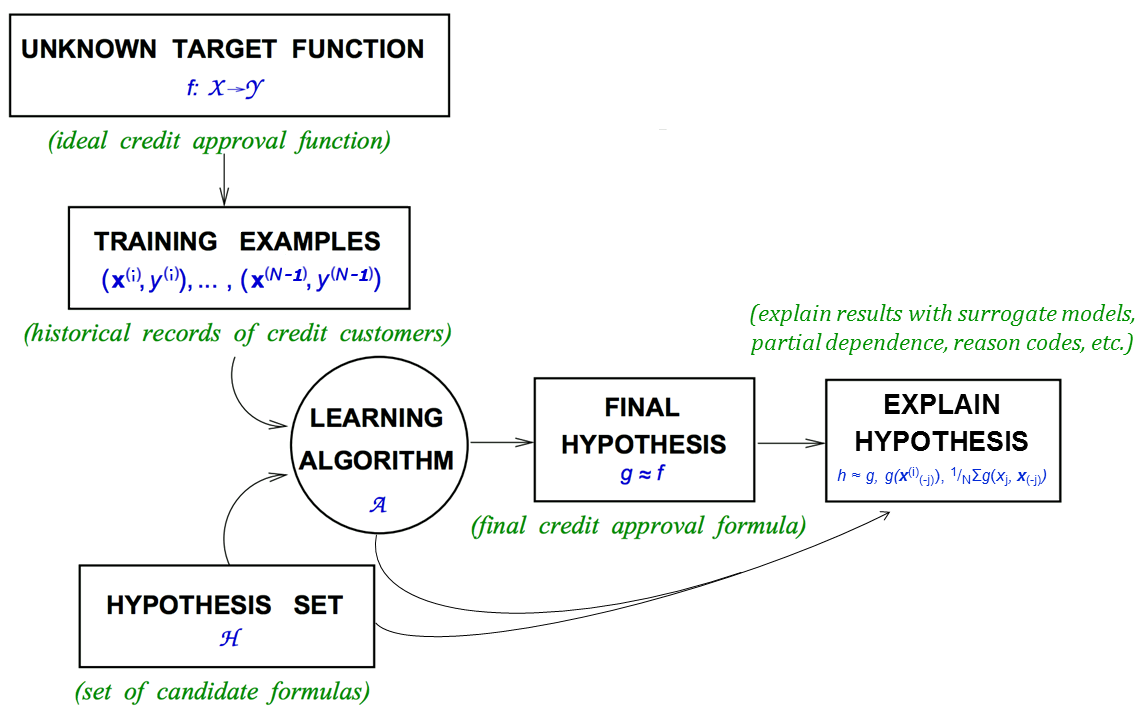
\includegraphics[height=140pt]{img/learning_problem.png}
		\label{fig:learning_problem}
		\caption{An augmented learning problem diagram in which several techniques create explanations for a credit scoring model. Adapted from \textbf{Learning From Data} \cite{lfd}.}
	\end{center}
\end{figure}	
	
As in Figure \ref{fig:learning_problem}, the presented explanatory methods help practicioners make random forests, GBMs, and other types of popular supervised  machine learning models more interpretable by enabling post-hoc explanations that are suitable for:\\

\begin{itemize}
	\item Facilitating regulatory compliance.
	\item Understanding or debugging model mechanisms and predictions.
	\item Preventing or debugging accidental or intentional discrimination in model predictions.
	\item Preventing or debugging malicious hacking of models or adversarial attacks on models.
\end{itemize}

Detailed discussions of the explanatory methods begin below by defining notation. Then sections \ref{sec:surrogate_dt} -- \ref{sec:shap} discuss explanatory methods and present recommendations for each method. Section \ref{sec:gen_rec} presents some general interpretability recommendations for practicioners. Section \ref{sec:suggested} discusses several additional interpretability subjects that are likely important for practicioners, and finally, section \ref{sec:software} highlights a few software resources that accompany this paper. 

%-------------------------------------------------------------------------------
\section{Notation} \label{sec:notation}
%-------------------------------------------------------------------------------

To facilitate technical descriptions of explanatory techniques, notation for input and output spaces, for datasets, and for models is defined.

\subsection{Spaces} 
 
	\begin{itemize}
		\item Input features come from a set $\mathcal{X}$ contained in a \textit{P}-dimensional input space, $\mathcal{X} \subset \mathbb{R}^P$.  
		\item Known labels corresponding to instances of $\mathcal{X}$ come from the set $\mathcal{Y}$ and are contained in a $C$-dimensional label space, $\mathcal{Y} \subset \mathbb{R}^C$.
		\item Learned output responses come from a set $\mathcal{\hat{Y}}$. For regression models, the set $\mathcal{\hat{Y}}_r$ is also contained in a $C$-dimensional output space, $\mathcal{\hat{Y}}_r \subset \mathbb{R}^{C_r}$. For classification models, the set $\mathcal{\hat{Y}}_c$ typically contains a column vector for each unique class in $\mathcal{Y}$. Hence, $\mathcal{\hat{Y}}_c$ is contained in a $C'$-dimensional output space,  $\mathcal{\hat{Y}}_c \subset \mathbb{R}^{C'_c}$.
	\end{itemize}	
	
\subsection{Datasets} 

	\begin{itemize}
		\item The input dataset $\mathbf{X}$ is composed of observed instances of the set $\mathcal{X}$ with a corresponding dataset of labels $\mathbf{Y}$, observed instances of the set $\mathcal{Y}$.
		\item Each $i$-th observation of $\mathbf{X}$ is denoted as $\mathbf{x}^{(i)} = $ \\ 
		$[x_0^{(i)}, x_1^{(i)}, \dots, x_{\textit{P}-1}^{(i)}]$, with corresponding $i$-th \\ labels in $\mathbf{Y}, \mathbf{y}^{(i)} = [y_0^{(i)}, y_1^{(i)}, \dots, y_{\textit{C}-1}^{(i)}]$.
		\item $\mathbf{X}$ and $\mathbf{Y}$ consists of $N$ tuples of observations:\\ $[(\mathbf{x}^{(0)},\mathbf{y}^{(0)}), (\mathbf{x}^{(1)},\mathbf{y}^{(1)}), \dots, (\mathbf{x}^{(N-1)},\mathbf{y}^{(N-1)})]$, \\ $\mathbf{x}^{(i)} \in \mathcal{X}$, $\mathbf{y}^{(i)} \in \mathcal{Y}$.
		\item Each $j$-th input column vector of $\mathbf{X}$ is denoted as $X_j = [x_{j}^{(0)}, x_{j}^{(1)}, \dots, x_{j}^{(N-1)}]^T$.
	\end{itemize}	 

\subsection{Models}

	\begin{itemize}
		\item A machine learning model $g$, selected from a hypothesis set $\mathcal{H}$, is trained to represent an unknown target function $f$ observed as  $\mathbf{X}$ with labels $\mathbf{Y}$ using a training algorithm $\mathcal{A}$: 
		$ \mathbf{X}, \mathbf{Y} \xrightarrow{\mathcal{A}} g$.
		\item $g$ generates learned output responses on the input dataset $g(\mathbf{X}) = \mathbf{\hat{Y}}$, and on the general input space $g(\mathcal{X}) = \mathcal{\hat{Y}}$.
		\item The model to be explained is denoted as $g$.
	\end{itemize}

%-------------------------------------------------------------------------------
\section{Surrogate Decision Trees} \label{sec:surrogate_dt}
%-------------------------------------------------------------------------------

% mention "proxy" and "shadow" 

\begin{figure}[htb]
	\begin{center}
		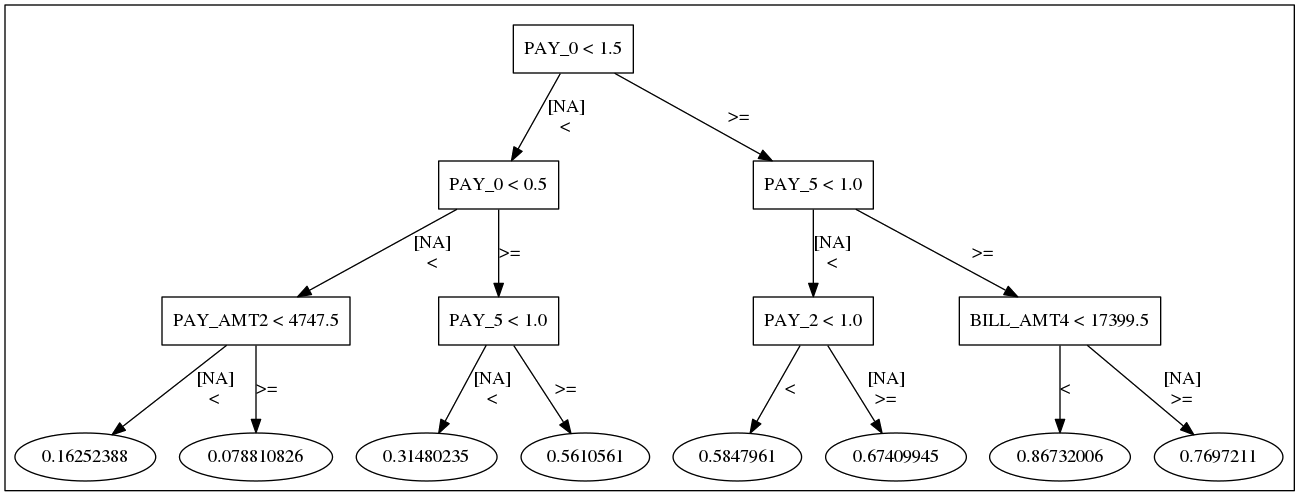
\includegraphics[height=90pt]{img/dt_surrogate.png}
		\label{fig:dt_surrogate}
		\caption{$h_{\text{tree}}$ for Taiwanese credit card data \cite{uci}, and for machine-learned GBM response function $g$.}
	\end{center}
\end{figure}

\begin{itemize}
	
	\item Given a learned function $g$ and set of predictions $g(\mathbf{X})$, a surrogate DT can be trained: $ \mathbf{X}, g(\mathbf{X}) \xrightarrow{\mathcal{A}_{\text{surrogate}}} h_{\text{tree}}$.
	
	\item $h_{\text{tree}}$ displays a low-fidelity, high-interpretability flow chart of $g$'s decision making process, and important features and interactions in $g$.	
	
\end{itemize}

\begin{itemize}
	
	\item Always use error measures to assess the trustworthiness of $h_{\text{tree}}$.
	
	\item Prescribed methods \cite{dt_surrogate1}; \cite{dt_surrogate2} for training $h_{\text{tree}}$ do exist. In practice, straightforward cross-validation approaches are typically sufficient. 
	
	\item Comparing cross-validated training error to traditional training error can give an indication of the stability of the single tree model, $h_{\text{tree}}$.
	
	\item \cite{lime-sup} use local linear surrogate models, $h_{\text{GLM}}$, in $h_{\text{tree}}$ leaf nodes to increase overall surrogate model fidelity while also retaining a high degree of interpretability.
	
\end{itemize}

%-------------------------------------------------------------------------------
\section{Partial Dependence and Individual Conditional Expectation (ICE) plots}
\label{sec:pd_ice}
%-------------------------------------------------------------------------------

\begin{itemize}
	
	\item Following \cite{esl} a single feature $X_j \in \mathbf{X}$ and its complement set $X_{(-j)} \in \mathbf{X}$ (where $X_j \cup X_{(-j)} = \mathbf{X}$) is considered.
	
	\item $\text{PD}(X_j, g)$ for a given feature $X_j$ is estimated as the average output of the learned function $g$ when all the components of $X_j$ are set to a constant $x \in \mathcal{X}$ and $X_{(-j)}$ is left untouched.
	
	\item $\text{ICE}(X_j, \mathbf{x}^{(i)}, g)$ for a given observation $\mathbf{x}^{(i)}$ and feature $X_j$ is estimated as the output of the learned function $g$ when $x^{(i)}_j$ is set to a constant $x \in \mathcal{X}$ and $\mathbf{x}^{(i)} \in X_{(-j)}$ are left untouched.
	
	\item PD and ICE curves are usually plotted over some set of interesting constants $x \in \mathcal{X}$. 

\end{itemize}

\begin{figure}[htb]
	\begin{center}
		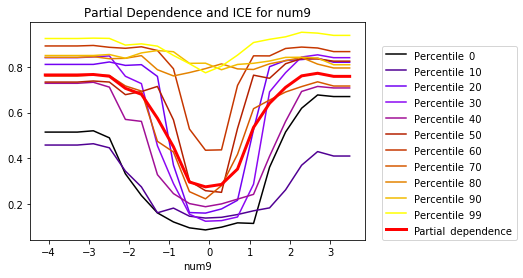
\includegraphics[height=100pt]{img/pdp_ice.png}
		\label{fig:pdp_ice}
		\caption{PD and ICE curves for $ X_j = \text{num}_9$, for known signal generating function $f(\mathbf{X}) = \text{num} _1 * \text{num}_4 + |\text{num}_8| * \text{num}_9^2 + e$, and for machine-learned GBM response function $g$.}
	\end{center}
\end{figure}

\vspace{-10pt}

Overlaying PD and ICE curves is a succinct method for describing global and local prediction behavior and can be used to detect interactions. \cite{ice_plots} 

\begin{figure}[htb]
	\begin{center}
		\label{fig:dt_surrogate_pdp_ice}
		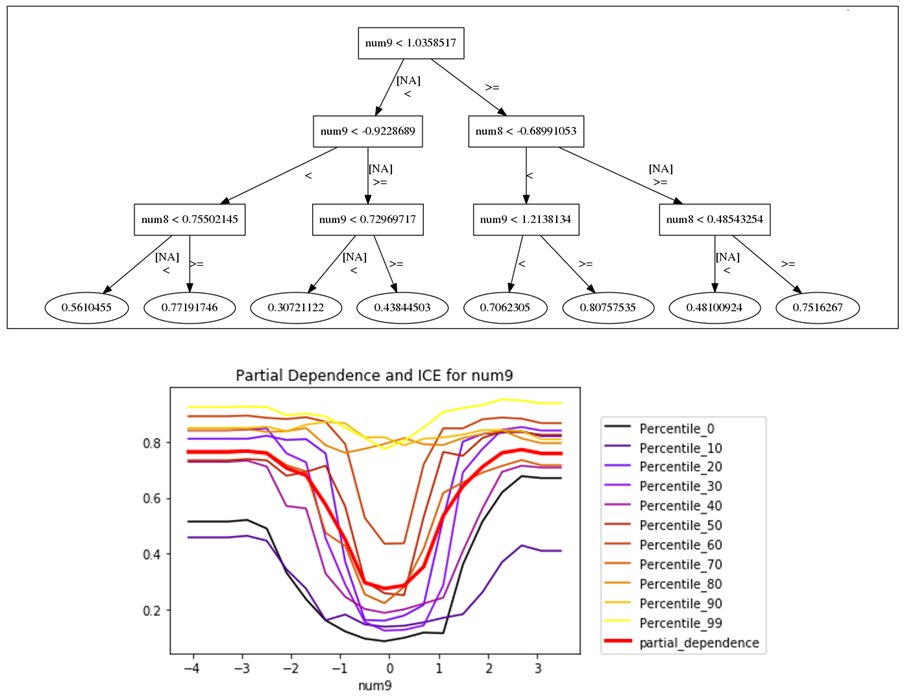
\includegraphics[height=190pt]{img/dt_surrogate2_pdp_ice.png}
		\caption{Surrogate DT, PD, and ICE curves for $ X_j = \text{num}_9$, for known signal generating function $f(\mathbf{X}) = \text{num} _1 * \text{num}_4 + |\text{num}_8| * \text{num}_9^2 + e$, and for machine-learned GBM response function $g$.}
	\end{center}
\end{figure}

Combining Surrogate DT models with PD and ICE curves is a convenient method for detecting, confirming, and understanding important interactions.

%-------------------------------------------------------------------------------
\section{Local Interpretable Model-agnostic Explanations (LIME)}
\label{sec:lime}
%-------------------------------------------------------------------------------

\cite{lime} defines LIME for some observation $\mathbf{x} \in \mathcal{X}$:

\begin{equation}
\begin{aligned}
\underset{h \in \mathcal{H}}{\arg\max}\:\mathcal{L}(g, h, \pi_{\mathbf{X}}) + \Omega(h)
\end{aligned}
\end{equation}

Here $g$ is the function to be explained, $h$ is an interpretable surrogate model of $g$, often a linear model $h_{GLM}$, $\pi_{\mathbf{X}}$ is a weighting function over the domain of $g$, and $\Omega(h)$ limits the complexity of $h$.

\vspace{5pt}

Typically, $h_{GLM}$ is constructed such that

\begin{equation}
\begin{aligned}
\mathbf{X}^{(*)}, g({X}^{(*)}) \xrightarrow{\mathcal{A}_{\text{surrogate}}} h_{\text{GLM}}
\end{aligned}
\end{equation}

where $\mathbf{X}^{(*)}$ is a generated sample, $\pi_{\mathbf{X}}$ weighs $\mathbf{X}^{(*)}$ samples by their Euclidean similarity to $\mathbf{x}$, local feature importance is estimated using $\beta_j x_j$, and $L_1$ regularization is used to induce a simplified, sparse $h_{GLM}$. 		

\begin{itemize}
	
	\item LIME is ideal for creating low-fidelity, highly interpretable explanations for non-DT models and for neural network models trained on unstructured data, e.g. deep learning.
	
	\item Always use regression fit measures to assess the trustworthiness of LIME explanations.
	
	\item LIME can be difficult to deploy, but there are highly deployable variants. \cite{lime-sup}; \cite{h2o_mli_booklet}
	
	\item Local feature importance values are offsets from a local intercept.
	
	\begin{itemize}
		
		\item Note that the intercept in LIME can account for the most important local phenomena.
		
		\item Generated LIME samples can contain large proportions of out-of-range data that can lead to unrealistic intercept values. 
		
	\end{itemize}
	
\end{itemize}

\begin{itemize}
	
	\item To increase the fidelity of LIME explanations, try LIME on discretized input features and on manually constructed interactions.
	
	\item Use cross-validation to construct standard deviations or even confidence intervals for local feature importance values.
	
	\item LIME can fail, particularly in the presence of extreme nonlinearity or high-degree interactions.
	
\end{itemize}

%-------------------------------------------------------------------------------
\section{Tree Shap} \label{sec:shap}
%-------------------------------------------------------------------------------

Shapley explanations are a class of additive, consistent local feature importance measures with long-standing theoretical support, \cite{shapley}. For some observation $\mathbf{x} \in \mathcal{X}$, Shapley explanations take the form:

\vspace{-5pt}

\begin{equation}
\begin{aligned}
\phi_0 + \sum_{j=0}^{j=\mathcal{P} - 1} \phi_j \mathbf{x}_j^\prime
\end{aligned}
\end{equation}

Here $\mathbf{x}^\prime \in \{0,1\}^\mathcal{P}$ is a binary representation of $\mathbf{x}$ where 0 indicates missingness. Each $\phi_j$ is the local feature importance value associated with $x_j$.

\begin{itemize}
	
	\item Calculating Shapley values directly is typically infeasible, but they can be estimated in different ways.
	
	\item Tree Shap is a specific implementation of Shapley explanations that leverages DT structures to disaggregrate the contribution of each $x_j$ to $g(\mathbf{x})$ in a DT or DT-based ensemble model. \cite{tree_shap}
	
\end{itemize}

\begin{itemize}
	
	\item Tree Shap is ideal for high-fidelity explanations of DT-based models, perhaps even in regulated applications.
	
	\item Local feature importance values are offsets from a global intercept.
	
	\item LIME can be constrained to become Shapley explanations, i.e. kernel shap.
	
	\item A similar, popular method known as \textit{treeinterpreter} appears untrustworthy when applied to GBM models. 
	
\end{itemize}

%-------------------------------------------------------------------------------
\section{General Recommendations} \label{sec:gen_rec}
%-------------------------------------------------------------------------------

\begin{itemize}
	
	\item Monotonically constrained XGBoost, Surrogate DT, PD and ICE plots, and Tree Shap are a direct and open source way to create an interpretable nonlinear model.
	
	\item Global and local explanatory techniques are often necessary to explain a model.
	
	\item Use simpler low-fidelity or sparse explanations to understand more accurate and complex high-fidelity explanations.  
	
	\item Seek consistent results across multiple explanatory techniques. 
	
	\item Methods relying on generated data are sometimes unpalatable to users. They want to understand \textit{their} data.
	
	\item Surrogate models can provide low-fidelity explanations for model mechanisms in original feature spaces if $g$ is defined to include feature extraction or engineering.
	
	\item To increase adoption, production deployment of explanatory methods must be straightforward.
	
\end{itemize}

%-------------------------------------------------------------------------------
\section{Suggested Reading} \label{sec:suggested}
%-------------------------------------------------------------------------------

\begin{itemize}
\item xNN derivatives, neural net-specific methods.
\item Accurate and interpretable classifiers.
\item Fairness.
\end{itemize} 

%-------------------------------------------------------------------------------
\section{Software Resources} \label{sec:software}
%-------------------------------------------------------------------------------

\sloppy

\textbf{Comparison of Explanatory Techniques on Simulated Data:}\\
\href{https://github.com/h2oai/mli-resources/tree/master/lime_shap_treeint_compare}{https://github.com/h2oai/mli-resources/tree/master/lime\_shap\_treeint\_compare}\\

\vspace{10pt}

\textbf{In-depth Explanatory Technique Examples:}\\
\href{https://github.com/jphall663/interpretable_machine_learning_with_python}{https://github.com/jphall663/interpretable\_\\machine\_learning\_with\_python}\\

\vspace{10pt}

\textbf{"Awesome" Machine Learning Interpretability Resource List:}\\
\href{https://github.com/jphall663/awesome-machine-learning-interpretability}{https://github.com/jphall663/awesome-machine-learning-interpretability}

\fussy

%-------------------------------------------------------------------------------
\section{Acknowledgements} 
%-------------------------------------------------------------------------------

% Mark Chan, Navdeep Gill, Lingyao, Leland, others? Zach Lipton Wen Phan Lauren Diperna

%----------------------------------------------------------------------
% References
%----------------------------------------------------------------------

\Urlmuskip=0mu plus 1mu\relax
\bibliographystyle{icml2013}
\bibliography{jsm_2018_paper}

\end{document} 



